\documentclass[aspectratio=169, 10pt]{beamer}

\usepackage{bm} % bold math
\usepackage{fontspec}
\usepackage{minted}
\usepackage{pgf-pie}
\usepackage{tikz}
\usepackage{graphicx}
\newcommand\sbullet[1][.5]{\mathbin{\vcenter{\hbox{\scalebox{#1}{$\bullet$}}}}}

% Custom commands and environments
\makeatletter
\newcommand\version[1]{\renewcommand\@version{#1}}
\newcommand\@version{}
\def\insertversion{\@version}

\newcommand\course[1]{\renewcommand\@course{#1}}
\newcommand\@course{}
\def\insertcourse{\@course}

\newcommand\coursetitle[1]{\renewcommand\@coursetitle{#1}}
\newcommand\@coursetitle{}
\def\insertcoursetitle{\@coursetitle}

\newcommand\lecturenumber[1]{\renewcommand\@lecturenumber{#1}}
\newcommand\@lecturenumber{}
\def\insertlecturenumber{\@lecturenumber}
\makeatother

\newcommand{\slidetitle}[1]{{\xbseries \large \structure{#1}} \bigskip}
\newcommand{\term}[1]{{\color{blue} #1}}
\newcommand{\leftspace}{\hspace{1em}}
\newcommand{\inlinearrow}{
  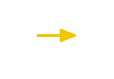
\begin{tikzpicture}[baseline]
    \node [anchor=base] (x) {};
    \draw [rawarrow] (x.mid west) -- ($(x.mid west) + (2em,0)$);
  \end{tikzpicture}
}

\newenvironment{slide}
{\begin{frame}[fragile,environment=slide]\vskip0pt plus 1filll}
{\vskip0pt plus 1filll\end{frame}}

% LaTeX

\setlength{\leftmargini}{1em}

% Common Information

\author{Talia Xu}
\course{COMPSCI 340}
\coursetitle{Operating Systems}
\date{2024 Semester 2}

% fontspec

\defaultfontfeatures{Ligatures=TeX}
% \setmainfont{Domine}
\setsansfont{Inter}[
  FontFace={ul}{n}{Font=*-Thin},
  FontFace={el}{n}{Font=*-ExtraLight},
  FontFace={l}{n}{Font=*-Light},
  FontFace={sb}{n}{Font=*-SemiBold},
  FontFace={eb}{n}{Font=*-ExtraBold},
  FontFace={xb}{n}{Font=*-Black},
]
\setmonofont[Contextuals=AlternateOff, Ligatures=TeXOff]{Iosevka}[
  FontFace={xb}{n}{Font=*-Heavy},
]

%% Font Weights

\DeclareRobustCommand{\ulseries}{\fontseries{ul}\selectfont}
\DeclareTextFontCommand{\textul}{\ulseries}
\DeclareRobustCommand{\elseries}{\fontseries{el}\selectfont}
\DeclareTextFontCommand{\textel}{\elseries}
\DeclareRobustCommand{\lseries}{\fontseries{l}\selectfont}
\DeclareTextFontCommand{\textl}{\lseries}
\DeclareRobustCommand{\sbseries}{\fontseries{sb}\selectfont}
\DeclareTextFontCommand{\textsb}{\sbseries}
\DeclareRobustCommand{\ebseries}{\fontseries{eb}\selectfont}
\DeclareTextFontCommand{\texteb}{\ebseries}
\DeclareRobustCommand{\xbseries}{\fontseries{xb}\selectfont}
\DeclareTextFontCommand{\textxb}{\xbseries}

% tikz

\usetikzlibrary{
  arrows,
  arrows.meta,
  automata,
  backgrounds,
  calc,
  decorations.pathreplacing,
  matrix,
  positioning,
  overlay-beamer-styles,
  shapes,
  shapes.multipart,
  tikzmark,
}

\tikzstyle{rawarrow} = [
  -{Latex[round]},
  line width=1pt,
  yellow,
  shorten >=3pt,
  shorten <=3pt,
  font=\small,
  text=black,
]

\tikzstyle{arrow} = [
  -{Latex[round]},
  line width=1pt,
  yellow,
  shorten >=3pt,
  shorten <=3pt,
  transform canvas={yshift=3pt},
  font=\small,
  text=black,
]

\newcommand{\tikzmarkcoord}[1]{([yshift=3pt]pic cs:#1)}

% minted

\setminted{style=eyolfson, fontsize=\small, escapeinside=||}
\setmintedinline{fontsize=\normalsize}

% hyperref

\hypersetup{colorlinks, urlcolor=blue}

% beamer
\setbeamersize{text margin left=16mm, text margin right=16mm}
\setbeamertemplate{itemize items}[circle]
\setbeamercolor{item}{fg=black}
\setbeamercolor{structure}{fg=darkblue}
\setbeamerfont{frametitle}{series=\bfseries, parent=structure}
\setbeamertemplate{navigation symbols}{}
\setbeamertemplate{headline}{}
\setbeamertemplate{footline}{
  \begin{tikzpicture}[
    remember picture,
    overlay,
    shift={(current page.south west)},
  ]
    \path [fill=gray] (144mm, 0) -- (160mm, 16mm) -- (160mm, 0);
    \node [inner sep=3.5mm, outer sep=0, text=black, anchor=base east,
           align=right, yshift=3.5mm]
          at (current page.south east) {\ttfamily \small \insertframenumber{}};
  \end{tikzpicture}
}
\setbeamertemplate{title page}{
  \begin{tikzpicture}[
    remember picture,
    overlay,
    shift={(current page.south west)},
    background rectangle/.style={fill=darkblue},
    show background rectangle,
  ]
    \node [anchor=center, align=center, text=white, text width=40mm, scale=3.2]
          at (\paperwidth / 2, \paperheight * 2 / 3)
          {\xbseries \inserttitle{}};
    \node [anchor=base west, align=left, inner sep=0, text=white, yshift=2.5mm]
          at (16mm, \paperheight / 3)
          {\insertdate{} \insertcourse{}: \insertcoursetitle{}};
    \node [anchor=base west, align=left, inner sep=0, text=white, yshift=-2.5mm]
          at (16mm, \paperheight / 3)
          {\insertauthor};
    \node [anchor=base east, align=right, inner sep=0, text=white, yshift=2.5mm]
          at (144mm, \paperheight / 3)
          {Lecture \insertlecturenumber{}};
    \node [anchor=base east, align=right, inner sep=0, text=white,
           yshift=-2.5mm]
          at (144mm, \paperheight / 3)
          {\ttfamily \insertversion{}};
    \node [align=center, anchor=south, inner sep=0, text=white, yshift=3.5mm]
          (license) at (\paperwidth / 2, 0)
          {\fontsize{7pt}{7pt}\selectfont This  work is licensed under a
           \href{http://creativecommons.org/licenses/by-sa/4.0/}
                {\color{lightblue} Creative Commons Attribution-ShareAlike 4.0
                 International License}};
  \end{tikzpicture}
}

% xcolor

%% Primary Colour

\definecolor{pantone655}{RGB}{0, 42, 92} % #002a5c
\colorlet{darkblue}{pantone655}

%% Secondary Colours

\definecolor{pantone633}{RGB}{0, 139, 176} % #008bb0
\colorlet{blue}{pantone633}

\definecolor{pantonewarmred}{RGB}{220, 70, 51} % #dc4633
\colorlet{red}{pantonewarmred}

\definecolor{pantone3285}{RGB}{0, 161, 137} % #00a189
\colorlet{cyan}{pantone3285}

\definecolor{pantone7722}{RGB}{13, 83, 77} % #0d534d
\colorlet{darkcyan}{pantone7722}

\definecolor{pantone376}{RGB}{141, 191, 46} % #8dbf2e
\colorlet{green}{pantone376}

\definecolor{pantone2613}{RGB}{109, 36, 122} % #6d247a
\colorlet{violet}{pantone2613}

\definecolor{pantone2985}{RGB}{111, 199, 234} % #6fc7ea
\colorlet{lightblue}{pantone2985}

\definecolor{pantone227}{RGB}{171, 19, 104} % #ab1368
\colorlet{magenta}{pantone227}

\definecolor{pantone7406}{RGB}{241, 197, 0} % #f1c500
\colorlet{yellow}{pantone7406}

%% Neutrals

\definecolor{pantonecoolgray2}{RGB}{208, 209, 201} % #d0d1c9
\colorlet{gray}{pantonecoolgray2}


\lecturenumber{1}
\title{File\\Systems}
\version{1.0.0}

\begin{document}

\begin{slide}
	Please sit close to the front of the class to help me save my voice =)
	\bigskip
	
	Please sit close to someone if possible for in-class discussions.
\end{slide}

\begin{frame}[plain, noframenumbering]
    \titlepage
\end{frame}

\begin{slide}
    \slidetitle{File system APIs}

    \textbf{Open}
    \begin{itemize}
        \item Open-file table: tracks open files
        \item File descriptor: pointer to last read/write location
        \item File-open count: counter of number of times a file is open
        \item Disk location of the file: cache of data access information
        \item Access rights: per-process access mode information
    \end{itemize}
    \medskip

    \textbf{Close}
    \begin{itemize}
        \item close() decreases the open count
        \item When the open count reaches zero, the file is no longer in use - allow removal of data from open-file table when last processes closes it
        \item create() and delete() are system calls that work with closed rather than open files
    \end{itemize}

\end{slide}

\begin{slide}

    \slidetitle{POSIX Filesystem}

    \begin{minted}{c}
int open(const char *pathname, int flags, mode_t mode);

// flags can specify which operations: O_RDWR,O_WRONLY, O_RDWR
// also: O_APPEND moves the position to the end of the file initially

int close(int fd);

// close() closes a file descriptor, so that it no longer 
// refers to any file and may be reused.

// returns 0 on success.
  \end{minted}
  
\end{slide}

\begin{slide}

    \slidetitle{File system APIs}

    \textbf{Create}
    
    \begin{minted}{c}
int creat(const char *pathname, mode_t mode);
    \end{minted}
    \bigskip

	\begin{minted}[fontsize=\scriptsize, escapeinside=]{console}
$ strace touch empty
execve("/usr/bin/touch", ["touch", "empty"], 0x7ffec0b50ca8 /* 62 vars */) = 0
...
openat(AT_FDCWD, "empty", O_WRONLY|O_CREAT|O_NOCTTY|O_NONBLOCK, 0666) = 3
...
utimensat(0, NULL, NULL, 0) = 0
	\end{minted}

\end{slide}

\begin{slide}

    \slidetitle{File system APIs}

    \textbf{Delete}
    \begin{minted}{c}
int unlink(const char *pathname);
    \end{minted}
	\medskip

	\begin{minted}[fontsize=\scriptsize, escapeinside=]{console}
$ strace rm empty_5mb.txt
openatexecve("/usr/bin/rm", ["rm", "empty_5mb.txt"], 0x7ffec6aa3788 /* 62 vars */) = 0
…

newfstatat(AT_FDCWD, "empty_5mb.txt", {st_mode=S_IFREG|0664, st_size=5242880, ...}, AT_SYMLINK_NOFOLLOW) = 0
faccessat2(AT_FDCWD, "empty_5mb.txt", W_OK, AT_EACCESS) = 0
unlinkat(AT_FDCWD, "empty_5mb.txt", 0) = 0
	\end{minted}

    \bigskip
    Is the deleted data overwritten?
    Is data recovery possible?
\end{slide}

\begin{slide}
    \slidetitle{Aside: What is a solid state drive (SSD)}?

    Use transistors (like RAM) to store data rather than magnetic disks.
    \bigskip

    \includegraphics[width=64mm]{ssd-hdd.jpg}

\end{slide}

\begin{slide}
  
    \slidetitle{SSDs are more modern}

    Pros
    \begin{itemize}
        \item No moving parts or physical limitations
        \item Higher throughput, and good random access
        \item More energy efficient
        \item Better space density
    \end{itemize}
    \medskip

    Cons
    \begin{itemize}
        \item More expensive
        \item Lower endurance (number of writes)
        \item More complicated to write drivers for
    \end{itemize}

\end{slide}

\begin{slide}
  
    \slidetitle{A SSD contains pages}

    Pages are typically 4 KB.

    \includegraphics[height=0.65\textheight]{ssd.png} 

\end{slide}


\begin{slide}
  
    \slidetitle{NAND Flash Programming Uses Pages and Blocks}

    You can only read complete pages and write to freshly erased pages
    \bigskip

    Erasing is done per block (a block has 128 or 256 pages)
    \begin{itemize}
        \item An entire block needs to be erased before writing
    \end{itemize}
    \bigskip

    Writing is slow (may need to create a new block)

\end{slide}

\begin{slide}
  
    \slidetitle{The OS Can Help Speed Up SSDs}

    SSDs need to garbage collect blocks
    \begin{itemize}
        \item Move any pages that are still alive to a new block (may be overhead)
    \end{itemize}
    \bigskip

    The disk controller doesn't know what blocks are still alive
    \begin{itemize}
        \item SSD may think the disk is full, when a file could be deleted (not erased)
    \end{itemize}
    \bigskip

    The OS can use the \textbf{TRIM} command to inform the SSD a block is unused
    \begin{itemize}
        \item The SSD can freely erase the block without moving overhead
    \end{itemize}

\end{slide}

\begin{slide}

    \slidetitle{TRIM}

    \includegraphics[height=0.75\textheight]{ssd-trim.png}

\end{slide}

\begin{slide}

    \slidetitle{Back to the API: delete()}

    Most modern computers use SDD.
    \bigskip

    Most modern OS has TRIM enabled by default.
    \bigskip

    Direct recovery is near impossible.
    \begin{itemize}
        \item Versioning file system
    \end{itemize}

\end{slide}

\begin{slide}

    \slidetitle{Storing files on disk}

    We have learned about creating and deleting files from the user side.
    \bigskip

    How is this implemented on the disk?
    \bigskip

    We will start by looking at a very simple file system (VSFS).

\end{slide}

\begin{slide}

    \slidetitle{A Very Simple File System (VSFS)}

    \includegraphics[width=100mm]{VSFS-1.png}
    \bigskip

    A disk is divided into a series of blocks. A common size is 4 KB (or 8).
    \bigskip

    What do we need to store in these blocks to build a file system?
    \bigskip

    In the beginning, every block is “empty” (not allocated).

\end{slide}

\begin{slide}

    \slidetitle{Example metadata}
    \bigskip

    \textbf{Core Attributes}
    \begin{itemize}
        \item Filename: The name used to identify the file.
        \item File Type: Indicates the type of file (e.g., text, image, video, executable, etc.).
        \item File Size: The size of the file in bytes.
        \item Permissions: Controls who can read, write, and execute the file (user, group, others).
        \item Ownership: Identifies the user and group that own the file.
    \end{itemize}
    \bigskip

    \textbf{Timestamps}
    \begin{itemize}
        \item Creation Time: When the file was created.
        \item Last Modified Time: When the file's content was last changed.
        \item Last Access Time: When the file was last opened or read.
    \end{itemize}

\end{slide}

\begin{slide}

    \slidetitle{A Very Simple File System (VSFS)}
    
    \includegraphics[width=100mm]{VSFS-2.png}
    \bigskip

    Metadata is stored in i-nodes (more on this later).
    \bigskip

    i-nodes are typically 128 bytes or \textit{256 bytes}.

    Each block is 4 bytes.
    \bigskip

    How many i-nodes can we have in our VSFS?
    \begin{itemize}
        \item What does this mean?
    \end{itemize}

\end{slide}

\begin{slide}

    \slidetitle{A Very Simple File System (VSFS)}

    \includegraphics[width=100mm]{VSFS-3.png}
    \bigskip

    Which i-node and data blocks are free?
    \begin{itemize}
        \item A bit map: each bit indicates whether the corresponding block is free (0) or in use (1)
    \end{itemize}
    \bigskip

    \textbf{Superblock}
    \begin{itemize}
        \item Number of inodes and data blocks
        \item Where does the inode table (array) begin?
        \item What file system is this?
    \end{itemize}

\end{slide}

\begin{slide}

    \slidetitle{
        An inode Describes a File System Object
                  
        (Files and Directories)
    }
    
    \medskip
    \includegraphics[width=130mm]{inode-struct.png}
    \bigskip

    There are 15 (disk) pointers (not memory!)
    \bigskip

    Each disk block is 4 KB.
    \bigskip

    If each pointer points to a disk block. What is the maximum file size?
\end{slide}

\begin{slide}

    \slidetitle{                                  
        An inode Describes a File System Object   
                                                        
        (Files and Directories)                   
    }                                             

    \includegraphics[width=130mm]{inode-struct-2.png}
    \bigskip

    \textbf{Indirect pointer:} Instead of pointing to a block that contains user data, it points to a block that contains more pointers.
    \bigskip

\end{slide}

\begin{slide}

    \slidetitle{                                  
        An inode Describes a File System Object   
                                                        
        (Files and Directories)                   
    }                                             

    \includegraphics[width=130mm]{inode-struct-2.png}
    \bigskip

    Assume each data block is 4 KB.

    Assume each pointer is 4 bytes.
    \bigskip

    What is the maximum file size of 12 direct pointers + 1 indirect pointer?

\end{slide}

\begin{slide}

    \slidetitle{                                  
        An inode Describes a File System Object   
                                                        
        (Files and Directories)                   
    }                                             

    \includegraphics[width=130mm]{inode-struct-2.png}
    \bigskip

    What is the maximum supported file size?

\end{slide}

\begin{slide}
    
    \slidetitle{How Do We Store Files? Contiguous Allocation?}
    
    \begin{center}       
		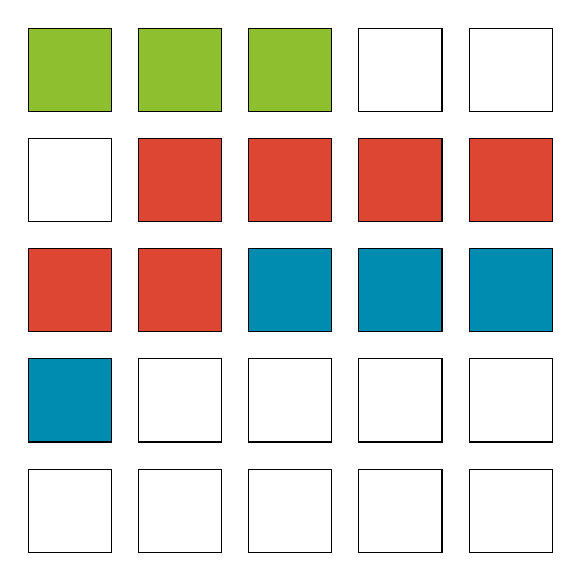
\begin{tikzpicture}[node distance=14mm and 14mm]

			\node[rectangle,draw,minimum width=30,minimum height=30,fill=pantone376] (b1)   {};
			\node[rectangle,draw,minimum width=30,minimum height=30,fill=pantone376] (b2) [right of=b1]  {};
			\node[rectangle,draw,minimum width=30,minimum height=30,fill=pantone376] (b3) [right of=b2]  {};
			\node[rectangle,draw,minimum width=30,minimum height=30] (b4) [right of=b3]  {};
			\node[rectangle,draw,minimum width=30,minimum height=30] (b5) [right of=b4]  {};

			\node[rectangle,draw,minimum width=30,minimum height=30] (b6) [below of=b1]  {};
			\node[rectangle,draw,minimum width=30,minimum height=30,fill=pantonewarmred] (b7) [right of=b6]  {};
			\node[rectangle,draw,minimum width=30,minimum height=30,fill=pantonewarmred] (b8) [right of=b7]  {};
			\node[rectangle,draw,minimum width=30,minimum height=30,fill=pantonewarmred] (b9) [right of=b8]  {};
			\node[rectangle,draw,minimum width=30,minimum height=30,fill=pantonewarmred] (b10) [right of=b9]  {};

			\node[rectangle,draw,minimum width=30,minimum height=30,fill=pantonewarmred] (b11) [below of=b6]  {};
			\node[rectangle,draw,minimum width=30,minimum height=30,fill=pantonewarmred] (b12) [right of=b11]  {};
			\node[rectangle,draw,minimum width=30,minimum height=30,fill=pantone633] (b13) [right of=b12]  {};
			\node[rectangle,draw,minimum width=30,minimum height=30,fill=pantone633] (b14) [right of=b13]  {};
			\node[rectangle,draw,minimum width=30,minimum height=30,fill=pantone633] (b15) [right of=b14]  {};

			\node[rectangle,draw,minimum width=30,minimum height=30,fill=pantone633] (b16) [below of=b11]  {};
			\node[rectangle,draw,minimum width=30,minimum height=30] (b17) [right of=b16]  {};
			\node[rectangle,draw,minimum width=30,minimum height=30] (b18) [right of=b17]  {};
			\node[rectangle,draw,minimum width=30,minimum height=30] (b19) [right of=b18]  {};
			\node[rectangle,draw,minimum width=30,minimum height=30] (b20) [right of=b19]  {};

			\node[rectangle,draw,minimum width=30,minimum height=30] (b21) [below of=b16]  {};
			\node[rectangle,draw,minimum width=30,minimum height=30] (b22) [right of=b21]  {};
			\node[rectangle,draw,minimum width=30,minimum height=30] (b23) [right of=b22]  {};
			\node[rectangle,draw,minimum width=30,minimum height=30] (b24) [right of=b23]  {};
			\node[rectangle,draw,minimum width=30,minimum height=30] (b25) [right of=b24]  {};
      \end{tikzpicture}
    \end{center}
 
\end{slide}

\begin{slide}
    
    \slidetitle{Contiguous Allocation Is Fast, If There Are No Modifications}

    Space efficient: Only start block and \# of blocks need to be stored
    \bigskip

    Fast random access: $block = floor(\frac{offset}{blocksize})$
    \bigskip

    Files can not grow easily
	\begin{itemize}
		\item Internal fragmentation (may not fill a block)
		\item External fragmentation when files are deleted or truncated
	\end{itemize}
	
\end{slide}

\begin{slide}
    
	\slidetitle{
		What About Storing Like a Free List of Pages?
    
		Linked Allocation
    }

    \begin{center}
		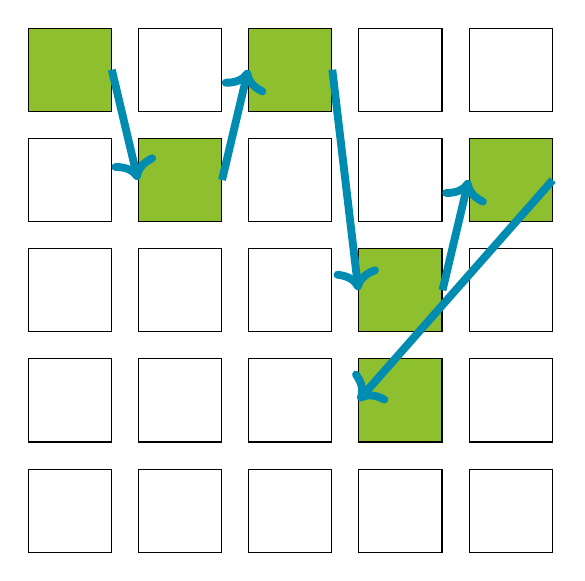
\begin{tikzpicture}[node distance=14mm and 14mm]
			\node[rectangle,draw,minimum width=30,minimum height=30,fill=pantone376] (b1)   {};
			\node[rectangle,draw,minimum width=30,minimum height=30] (b2) [right of=b1]  {};
			\node[rectangle,draw,minimum width=30,minimum height=30,fill=pantone376] (b3) [right of=b2]  {};
			\node[rectangle,draw,minimum width=30,minimum height=30] (b4) [right of=b3]  {};
			\node[rectangle,draw,minimum width=30,minimum height=30] (b5) [right of=b4]  {};

			\node[rectangle,draw,minimum width=30,minimum height=30] (b6) [below of=b1]  {};
			\node[rectangle,draw,minimum width=30,minimum height=30,fill=pantone376] (b7) [right of=b6]  {};
			\node[rectangle,draw,minimum width=30,minimum height=30] (b8) [right of=b7]  {};
			\node[rectangle,draw,minimum width=30,minimum height=30] (b9) [right of=b8]  {};
			\node[rectangle,draw,minimum width=30,minimum height=30,fill=pantone376] (b10) [right of=b9]  {};

			\node[rectangle,draw,minimum width=30,minimum height=30] (b11) [below of=b6]  {};
			\node[rectangle,draw,minimum width=30,minimum height=30] (b12) [right of=b11]  {};
			\node[rectangle,draw,minimum width=30,minimum height=30] (b13) [right of=b12]  {};
			\node[rectangle,draw,minimum width=30,minimum height=30,fill=pantone376] (b14) [right of=b13]  {};
			\node[rectangle,draw,minimum width=30,minimum height=30] (b15) [right of=b14]  {};

			\node[rectangle,draw,minimum width=30,minimum height=30] (b16) [below of=b11]  {};
			\node[rectangle,draw,minimum width=30,minimum height=30] (b17) [right of=b16]  {};
			\node[rectangle,draw,minimum width=30,minimum height=30] (b18) [right of=b17]  {};
			\node[rectangle,draw,minimum width=30,minimum height=30,fill=pantone376] (b19) [right of=b18]  {};
			\node[rectangle,draw,minimum width=30,minimum height=30] (b20) [right of=b19]  {};

			\node[rectangle,draw,minimum width=30,minimum height=30] (b21) [below of=b16]  {};
			\node[rectangle,draw,minimum width=30,minimum height=30] (b22) [right of=b21]  {};
			\node[rectangle,draw,minimum width=30,minimum height=30] (b23) [right of=b22]  {};
			\node[rectangle,draw,minimum width=30,minimum height=30] (b24) [right of=b23]  {};
			\node[rectangle,draw,minimum width=30,minimum height=30] (b25) [right of=b24]  {};

			\draw[->,line width=1mm,draw=pantone633] (b1.east) -- (b7.west);
			\draw[->,line width=1mm,draw=pantone633] (b7.east) -- (b3.west);
			\draw[->,line width=1mm,draw=pantone633] (b3.east) -- (b14.west);
			\draw[->,line width=1mm,draw=pantone633] (b14.east) -- (b10.west);
			\draw[->,line width=1mm,draw=pantone633] (b10.east) -- (b19.west);
		\end{tikzpicture}
    \end{center}
\end{slide}

\begin{slide}
    
    \slidetitle{Linked Allocation Has Slow Random Access}
    
    Space efficient: Only start block needs to be stored
	\begin{itemize}
		\item Blocks need to store a pointer to the next block (block is slightly smaller)
	\end{itemize}
    \bigskip

    Files can grow/shrink
	\begin{itemize}
		\item No external fragmentation
		\item
	\end{itemize}
	\bigskip

    How can we increase random access speed? We need to walk each block
	\begin{itemize}
		\item Each block may be located far away (it will never be cached)
	\end{itemize}

\end{slide}

\begin{slide}

    \slidetitle{File Allocation Table Moves The List to a Separate Table}
    
    \begin{center}      
		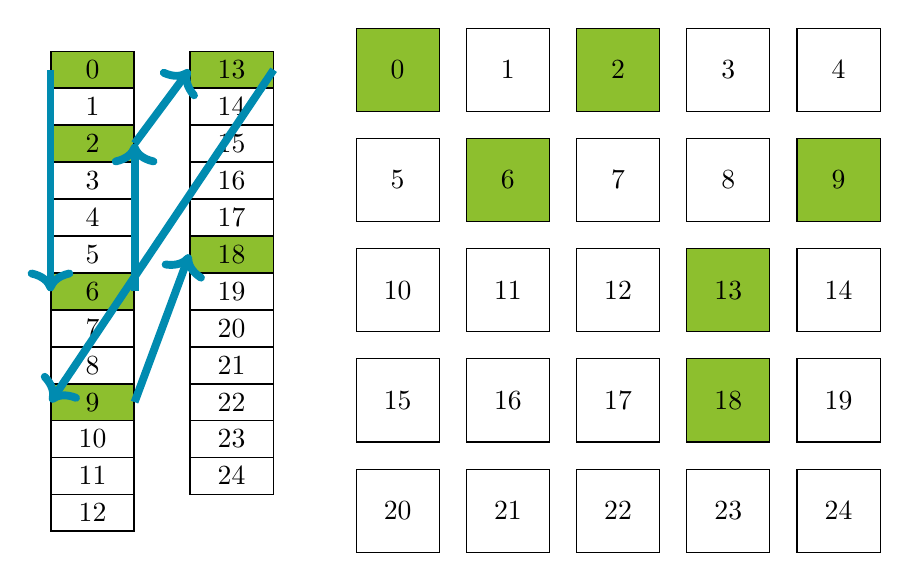
\begin{tikzpicture}[node distance=14mm and 14mm]
			\node[rectangle,draw,minimum width=30,minimum height=30,fill=pantone376] (b1)   {0};
			\node[rectangle,draw,minimum width=30,minimum height=30] (b2) [right of=b1]  {1};
			\node[rectangle,draw,minimum width=30,minimum height=30,fill=pantone376] (b3) [right of=b2]  {2};
			\node[rectangle,draw,minimum width=30,minimum height=30] (b4) [right of=b3]  {3};
			\node[rectangle,draw,minimum width=30,minimum height=30] (b5) [right of=b4]  {4};

			\node[rectangle,draw,minimum width=30,minimum height=30] (b6) [below of=b1]  {5};
			\node[rectangle,draw,minimum width=30,minimum height=30,fill=pantone376] (b7) [right of=b6]  {6};
			\node[rectangle,draw,minimum width=30,minimum height=30] (b8) [right of=b7]  {7};
			\node[rectangle,draw,minimum width=30,minimum height=30] (b9) [right of=b8]  {8};
			\node[rectangle,draw,minimum width=30,minimum height=30,fill=pantone376] (b10) [right of=b9]  {9};

			\node[rectangle,draw,minimum width=30,minimum height=30] (b11) [below of=b6]  {10};
			\node[rectangle,draw,minimum width=30,minimum height=30] (b12) [right of=b11]  {11};
			\node[rectangle,draw,minimum width=30,minimum height=30] (b13) [right of=b12]  {12};
			\node[rectangle,draw,minimum width=30,minimum height=30,fill=pantone376] (b14) [right of=b13]  {13};
			\node[rectangle,draw,minimum width=30,minimum height=30] (b15) [right of=b14]  {14};

			\node[rectangle,draw,minimum width=30,minimum height=30] (b16) [below of=b11]  {15};
			\node[rectangle,draw,minimum width=30,minimum height=30] (b17) [right of=b16]  {16};
			\node[rectangle,draw,minimum width=30,minimum height=30] (b18) [right of=b17]  {17};
			\node[rectangle,draw,minimum width=30,minimum height=30,fill=pantone376] (b19) [right of=b18]  {18};
			\node[rectangle,draw,minimum width=30,minimum height=30] (b20) [right of=b19]  {19};

			\node[rectangle,draw,minimum width=30,minimum height=30] (b21) [below of=b16]  {20};
			\node[rectangle,draw,minimum width=30,minimum height=30] (b22) [right of=b21]  {21};
			\node[rectangle,draw,minimum width=30,minimum height=30] (b23) [right of=b22]  {22};
			\node[rectangle,draw,minimum width=30,minimum height=30] (b24) [right of=b23]  {23};
			\node[rectangle,draw,minimum width=30,minimum height=30] (b25) [right of=b24]  {24};

			\node[rectangle,draw,minimum width=30,minimum height=10,xshift=-40,fill=pantone376] (fat1) [left=of b1] {0};
			\node[rectangle,draw,minimum width=30,minimum height=10,yshift=40] (fat2) [below=of fat1] {1};
			\node[rectangle,draw,minimum width=30,minimum height=10,yshift=40,fill=pantone376] (fat3) [below=of fat2] {2};
			\node[rectangle,draw,minimum width=30,minimum height=10,yshift=40] (fat4) [below=of fat3] {3};
			\node[rectangle,draw,minimum width=30,minimum height=10,yshift=40] (fat5) [below=of fat4] {4};
			\node[rectangle,draw,minimum width=30,minimum height=10,yshift=40] (fat6) [below=of fat5] {5};
			\node[rectangle,draw,minimum width=30,minimum height=10,yshift=40,fill=pantone376] (fat7) [below=of fat6] {6};
			\node[rectangle,draw,minimum width=30,minimum height=10,yshift=40] (fat8) [below=of fat7] {7};
			\node[rectangle,draw,minimum width=30,minimum height=10,yshift=40] (fat9) [below=of fat8] {8};
			\node[rectangle,draw,minimum width=30,minimum height=10,yshift=40,fill=pantone376] (fat10) [below=of fat9] {9};
			\node[rectangle,draw,minimum width=30,minimum height=10,yshift=40] (fat11) [below=of fat10] {10};
			\node[rectangle,draw,minimum width=30,minimum height=10,yshift=40] (fat12) [below=of fat11] {11};
			\node[rectangle,draw,minimum width=30,minimum height=10,yshift=40] (fat13) [below=of fat12] {12};

			\node[rectangle,draw,minimum width=30,minimum height=10,xshift=-20,fill=pantone376] (fat14) [right=of fat1] {13};
			\node[rectangle,draw,minimum width=30,minimum height=10,yshift=40] (fat15) [below=of fat14] {14};

			\node[rectangle,draw,minimum width=30,minimum height=10,yshift=40] (fat16) [below=of fat15] {15};
			\node[rectangle,draw,minimum width=30,minimum height=10,yshift=40] (fat17) [below=of fat16] {16};
			\node[rectangle,draw,minimum width=30,minimum height=10,yshift=40] (fat18) [below=of fat17] {17};
			\node[rectangle,draw,minimum width=30,minimum height=10,yshift=40,fill=pantone376] (fat19) [below=of fat18] {18};
			\node[rectangle,draw,minimum width=30,minimum height=10,yshift=40] (fat20) [below=of fat19] {19};
			\node[rectangle,draw,minimum width=30,minimum height=10,yshift=40] (fat21) [below=of fat20] {20};
			\node[rectangle,draw,minimum width=30,minimum height=10,yshift=40] (fat22) [below=of fat21] {21};
			\node[rectangle,draw,minimum width=30,minimum height=10,yshift=40] (fat23) [below=of fat22] {22};
			\node[rectangle,draw,minimum width=30,minimum height=10,yshift=40] (fat24) [below=of fat23] {23};
			\node[rectangle,draw,minimum width=30,minimum height=10,yshift=40] (fat25) [below=of fat24] {24};

			\draw[->,line width=1mm,color=pantone633] (fat1.west) -- (fat7.west);
			\draw[->,line width=1mm,color=pantone633] (fat7.east) -- (fat3.east);
			\draw[->,line width=1mm,color=pantone633] (fat3.east) -- (fat14.west);
			\draw[->,line width=1mm,color=pantone633] (fat14.east) -- (fat10.west);
			\draw[->,line width=1mm,color=pantone633] (fat10.east) -- (fat19.west);
		\end{tikzpicture}
    \end{center}

\end{slide}

\begin{slide}
    
    \slidetitle{File Allocation Table (FAT) is Similar to Linked Allocation}

    Files can grow/shrink
	\begin{itemize}
		\item No external fragmentation
		\item Internal fragmentation
	\end{itemize}
    \bigskip

    Fast random access: FAT can be held in memory/cache
    \begin{itemize}
		\item FAT size is linear to disk size: can become very large
	\end{itemize}
    \bigskip

    How can we further increase random access speed?

  \end{slide}

\begin{slide}
    
    \slidetitle{Indexed Allocation Maps Each Block Directly}

    \begin{center}
		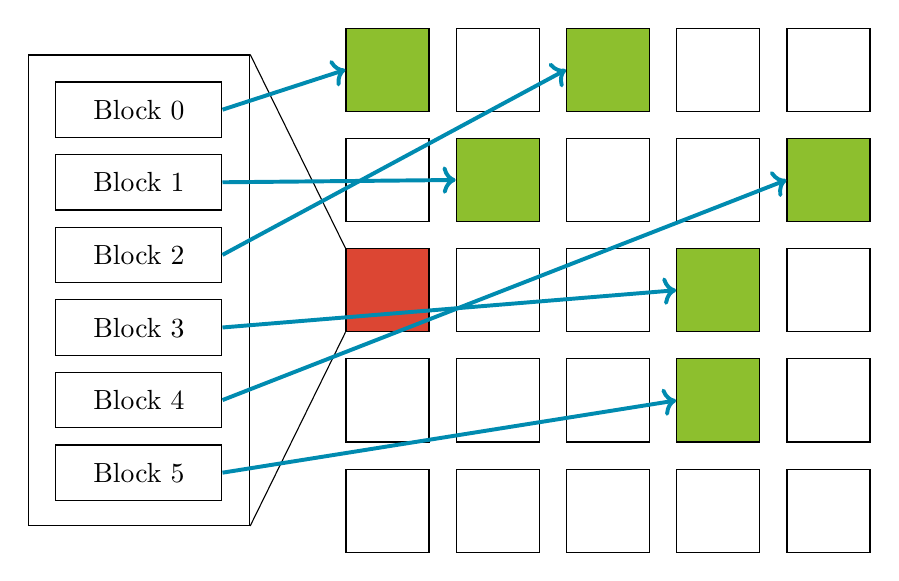
\begin{tikzpicture}[node distance=14mm and 14mm]
			\node[rectangle,draw,minimum width=30,minimum height=30,fill=pantone376] (b1)   {};
			\node[rectangle,draw,minimum width=30,minimum height=30] (b2) [right of=b1]  {};
			\node[rectangle,draw,minimum width=30,minimum height=30,fill=pantone376] (b3) [right of=b2]  {};
			\node[rectangle,draw,minimum width=30,minimum height=30] (b4) [right of=b3]  {};
			\node[rectangle,draw,minimum width=30,minimum height=30] (b5) [right of=b4]  {};

			\node[rectangle,draw,minimum width=30,minimum height=30] (b6) [below of=b1]  {};
			\node[rectangle,draw,minimum width=30,minimum height=30,fill=pantone376] (b7) [right of=b6]  {};
			\node[rectangle,draw,minimum width=30,minimum height=30] (b8) [right of=b7]  {};
			\node[rectangle,draw,minimum width=30,minimum height=30] (b9) [right of=b8]  {};
			\node[rectangle,draw,minimum width=30,minimum height=30,fill=pantone376] (b10) [right of=b9]  {};

			\node[rectangle,draw,minimum width=30,minimum height=30,fill=pantonewarmred] (b11) [below of=b6]  {};
			\node[rectangle,draw,minimum width=30,minimum height=30] (b12) [right of=b11]  {};
			\node[rectangle,draw,minimum width=30,minimum height=30] (b13) [right of=b12]  {};
			\node[rectangle,draw,minimum width=30,minimum height=30,fill=pantone376] (b14) [right of=b13]  {};
			\node[rectangle,draw,minimum width=30,minimum height=30] (b15) [right of=b14]  {};

			\node[rectangle,draw,minimum width=30,minimum height=30] (b16) [below of=b11]  {};
			\node[rectangle,draw,minimum width=30,minimum height=30] (b17) [right of=b16]  {};
			\node[rectangle,draw,minimum width=30,minimum height=30] (b18) [right of=b17]  {};
			\node[rectangle,draw,minimum width=30,minimum height=30,fill=pantone376] (b19) [right of=b18]  {};
			\node[rectangle,draw,minimum width=30,minimum height=30] (b20) [right of=b19]  {};

			\node[rectangle,draw,minimum width=30,minimum height=30] (b21) [below of=b16]  {};
			\node[rectangle,draw,minimum width=30,minimum height=30] (b22) [right of=b21]  {};
			\node[rectangle,draw,minimum width=30,minimum height=30] (b23) [right of=b22]  {};
			\node[rectangle,draw,minimum width=30,minimum height=30] (b24) [right of=b23]  {};
			\node[rectangle,draw,minimum width=30,minimum height=30] (b25) [right of=b24]  {};

			\node[rectangle,draw,minimum width=80,minimum height=170,xshift=-50] (index) [left of=b11]  {};
			\node[rectangle,draw,minimum width=60,minimum height=20,yshift=-70] (index1) [above=of index] {Block 0};
			\node[rectangle,draw,minimum width=60,minimum height=20,yshift=34] (index2) [below=of index1] {Block 1};
			\node[rectangle,draw,minimum width=60,minimum height=20,yshift=34] (index3) [below=of index2] {Block 2};
			\node[rectangle,draw,minimum width=60,minimum height=20,yshift=34] (index4) [below=of index3] {Block 3};
			\node[rectangle,draw,minimum width=60,minimum height=20,yshift=34] (index5) [below=of index4] {Block 4};
			\node[rectangle,draw,minimum width=60,minimum height=20,yshift=34] (index6) [below=of index5] {Block 5};

			\draw[-] (index.north east) -- (b11.north west);
			\draw[-] (index.south east) -- (b11.south west);

			\draw[->,line width=0.5mm,color=pantone633] (index1.east) -- (b1.west);
			\draw[->,line width=0.5mm,color=pantone633] (index2.east) -- (b7.west);
			\draw[->,line width=0.5mm,color=pantone633] (index3.east) -- (b3.west);
			\draw[->,line width=0.5mm,color=pantone633] (index4.east) -- (b14.west);
			\draw[->,line width=0.5mm,color=pantone633] (index5.east) -- (b10.west);
			\draw[->,line width=0.5mm,color=pantone633] (index6.east) -- (b19.west);
		\end{tikzpicture}
    \end{center}
\end{slide}

\begin{slide}
    
    \slidetitle{For Indexed Allocation, Each File Needs an Index Block}

    Files can still grow/shrink
	\begin{itemize}
		\item No external fragmentation
		\item Internal fragmentation
	\end{itemize}
    \bigskip

    Fast random access
    \bigskip

    File size limited by the maximum size of the index block (fit it in one block)

\end{slide}

\begin{slide}

    \slidetitle{Reading}

    Textbook 
    \begin{itemize}
        \item 14.4 Allocation Methods
    \end{itemize}
\end{slide}

\end{document}
